\section{Hearts Game Logic}

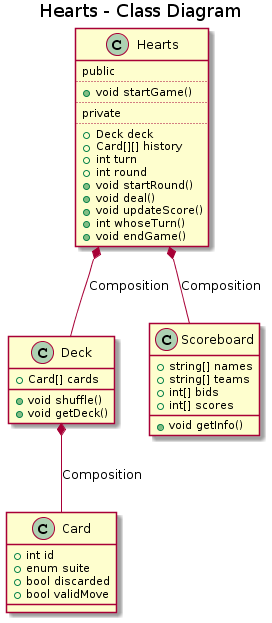
\includegraphics[scale=.85]{HeartsGameLogic/Hearts_Class_diagram.png}

\subsection{Hearts Class}

\subsubsection{Deck deck}
	Object deck which holds an array of 52 cards.
\subsubsection{Card[][] history}
	Array holds previous cards in play, allows client to view history.
\subsubsection{int turn}
	Variable to hold turn number for use in game logic.
\subsubsection{int round}
	Variable to hold round number for use in game logic.
\subsubsection{void startRound()}
	Start round will first update each client with their hands and then ask which cards need to be passed, it then will call a private function take turn.  
\subsubsection{void deal()}
	This function gives each player the appropriate cards at the beginning of each game or round.
\subsubsection{void updateScore()}
	This function updates the score after each player goes (or after each round depending on specific game)
\subsubsection{void whoseTurn()}
	This function keeps track of which player is next to play.
\subsubsection{void endGame()}
	This function allows the client to exit or play an additional game.

\subsection{Scoreboard Class}

\subsubsection{string[] names}
	String of player name.
\subsubsection{string[] teams}
	String of team player is on.
\subsubsection{int bids}
	Int of player bid.
\subsubsection{int scores}
	Int of player score.
\subsubsection{void getInfo()}
	This function calculates and updates information needed for displaying score for player.

\subsection{Deck Class}

\subsubsection{Card[] cards}
	This is an array (of size 52) of card objects to be used in a game.
\subsubsection{void shuffle()}
	This function changes the id values to different array elements to randomize a deck to be played in a game.
\subsubsection{void getDeck()}
	This allows the game logic to pull the information of the Deck class and use it for a game.
\subsection{Card Class}

\subsubsection{int id}
	This variable represents and corresponds to a specific card in a standard playing deck.
\subsubsection{enum suite}
	The card object will be one of four suites, enumerated to represent hearts, diamonds, spades, and clubs.
\subsubsection{bool discarded}
	This indicates whether a card has been discarded or played in a game.
\subsubsection{bool validMove}
	This indicates whether a card is playable in the current hand of play.
\end{document}
